%!TEX root = ../template.tex
%%%%%%%%%%%%%%%%%%%%%%%%%%%%%%%%%%%%%%%%%%%%%%%%%%%%%%%%%%%%%%%%%%%
%% chapter1.tex
%% NOVA thesis document file
%%
%% Chapter with introduction
%%%%%%%%%%%%%%%%%%%%%%%%%%%%%%%%%%%%%%%%%%%%%%%%%%%%%%%%%%%%%%%%%%%

\typeout{NT FILE chapter1.tex}%

\chapter{Introdução}
\label{cha:introduction}

\prependtographicspath{{Chapters/Figures/Covers/}}

% epigraph configuration
\epigraphfontsize{\small\itshape}
\setlength\epigraphwidth{12.5cm}
\setlength\epigraphrule{0pt}

\noindent Este capítulo tem como objetivo introduzir o tema da dissertação a ser desenvolvida. 
É apresentada a motivação para a realização do projeto, o contexto em que o problema abordado se insere e os objetivos a serem alcançados. 

\section{Motivação}
\label{sec:motivation}

Nos dias de hoje, a crescente inovação da tecnologia fez com que o comportamento dos consumidores fosse alterado. 
Dada a facilidade com que os consumidores estão sempre conectados à Internet, é visível um crescimento de serviços online, reduzindo deslocações e, deste modo, facilitando 
a vida dos mesmos. Estas mudanças impõe também a revolução das empresas e na forma como agem com os utilizadores \cite{LuisMarineYousef}\cite{Uma}. 
Serviços como a renovação do passaporte, que antes dependiam de deslocações a instalações físicas, estão rapidamente a ser substituídos por opções digitais, 
capazes de tornar todo o processo mais eficiente, acessível e conveniente. Para isto, é necessário garantir uma boa interação entre os cidadãos e os sistemas digitais.

De forma a minimizar as dúvidas dos consumidores e resolver os seus problemas, um apoio ao cliente forte é algo necessário e uma das soluções criadas 
para tornar este processo mais autónomo foi a utilização de chatbots, estes que se tornaram bastante comuns devido ao seu custo reduzido e o facto de 
conseguirem lidar com vários utilizadores simultaneamente.
Um chatbot consiste num programa de inteligência artificial que tem como objetivo simular uma conversa humana. Para isso, utiliza um processador de linguagem natural
(\textit{Natural Language Processing, NLP}), de forma a compreender as questões do utilizador \cite{Eleni}. 
Através de chatbots, as empresas conseguem garantir um atendimento mais rápido a todos os consumidores e dar uma experiência mais personalizada, tratando-se, por exemplo, 
de uma solução mais atrativa que as \textit{frequently asked questions} (FAQs). Os chatbots apresentam uma solução que oferece mais conforto e assistência aos 
utilizadores, dando repostas diretas aos seus problemas \cite{AdamopoulouMoussiades}.

Contudo, as abordagens tradicionais dos chatbots, baseadas em regras e fluxos predefinidos, têm as suas limitações. 
Estes sistemas são, por vezes, incapazes de lidar com a complexidade e ambiguidade da comunicação humana, o que resulta, muitas vezes, em frustações para os utilizadores, 
que recebem respostas imprecisas, não vendo assim os seus problemas resolvidos.
O futuro dos chatbots passa por reduzir estas limitações e fazer com que estes avancem para além de respostas estáticas, tornando-se sistemas dinâmicos \cite{Avyay}, 
capazes de interpretar pedidos complexos,
identificar o contexto e intenção do e de executar pedidos do utilizador, com base na interação textual ou verbal.

É neste contexto que surgem os \textit{Large Language Models} (\textit{LLMs}), sendo uma das inovações mais promissoras na área da inteligência artifical. 
Estes modelos, treinados a partir de uma vasta quantidade de dados, destacam-se pela sua capacidade para compreender, interpretar e gerar texto em linguagem natural, 
permitindo interações mais fluidas e próximas do diálogo humano. A integração dos \textit{LLMs} nos chatbots permite superar muitas das limitações associadas aos sistemas
tradicionais, uma vez que são capazes de interpretar e identificar as intenções do utilizador, permintindo contextualizar as respostas \cite{Sumit}.
Os \textit{LLMs} são, por isso, um passo fundamental para tornar os chatbots sistemas mais úteis e eficazes, aumentando o grau de satisfação do utilizador.

\section{Contexto}
\label{sec:context}

(FALTAM COISAS/ALTERAR)

Esta tese está integrada nas soluções desenvolvidas pela Opensoft, com o objetivo de otimizar o atendimento remoto através de tecnologias inovadoras. 

Atualmente, as soluções da Opensoft, como o idfyme, destacam-se por permitir que serviços que antes exigiam deslocações físicas, possam ser realizados digitalmente,
de forma a garantir acessibilidade aos cidadãos.

A proposta central desta tese visa desenvolver um chatbot capaz de interpretar linguagem natural e realizar tarefas em consequência, solicitando parâmetros quando necessário.
A integração deste chatbot nas soluções da Opensoft reforçam o compromisso da empresa na inovação tecnológica, respondendo à crescente necessidade da transformação digital.

\section{Objetivos}
\label{sec:objetivos}

O propósito central desta tese é desenvolver um chatbot inteligente, capaz de interpretar linguagem natural textual e executar automaticamente ações, com o objetivo de melhorar
significativamente a eficiência e experiênciada interação com o utilizador. Desta forma, o chatbot deve ser capaz de compreender as intenções dos utilizadores e de 
lidar com a ambiguidade da linguagem humana, fornecendo respostas contextualizadas e uma experiência personalizada. 

O projeto visa criar um chatbot que possa ser encorporado em soluções já existentes, oferecendo funcionalidades que complementam os serviços de atendimento digital.
Será também desenvolvida toda a \textit{User Interface} (\textit{UI}) do chatbot, com a finalidade de ser uma solução completa e pronta a utilizar. 

Além disso, pretende-se que o chatbot suporte também a integração com sistemas de back-office, possibilitando a automação de tarefas administrativas e a otimização
dos recursos humanos. O chatbot deverá ser seguro, garantindo a integridade e e confidencialidade das informações tratadas.

Adicionalmente, deverá ser estudada a hipótese do chatbot funcionar através de comandos voz, permitindo que os utilizadores interajam com o sistema de forma ainda mais
natural e conveniente. Esta adição faria com que fosse proporcionada uma experiência inclusiva e adaptada a diferentes perfis de utilizadores, podendo a solução chegar
a um público maior.

\section{Organização}
\label{sec:organization}

O documento está organizado nos seguintes capítulos:
\begin{enumerate}
  \item \textbf{Introdução - } Neste capítulo, é definida a motivação e contexto da dissertação, bem como os seus objetivos.
  \item \textbf{Estado da Arte - } Neste capítulo, é apresentado o estado da arte. São estudadas soluções semelhantes já existentes e apresentados conceitos importantes para a compreensão desta dissertação.
  \item \textbf{Tecnologias - } Neste capítulo, são apresentadas ferramentas estudadas para a elaboração da solução.   
  \item \textbf{Solução Proposta - } Neste capítulo, é apresentada a solução (descrição, tecnologias a usar, plano de trabalhos, requisitos da solução).
\end{enumerate}

The \gls{novathesis} template was born in~1996, and what you see now accumulates to many many hundreds (thousands?!) of working hours, unpaid and stolen from family and friends.  This work is available to the community under the \href{LaTeX project public license}{\LaTeX\ Project Public License v1.3c}, which means you are entitled to use it for free and change it at your will.  However, if you decide to use this template to write your thesis/dissertation, \textbf{be fair to the developers} and:
\begin{enumerate}
  \item \ntindex[novathesis!Citation]{} Cite the \gls{novathesis} manual~\cite{novathesis-manual} in a place of your choice (e.g., in the \emph{Acknowledgments}) of your thesis/dissertation with “\verb!\cite{novathesis-manual}!” .  If you cite it this way, the correct entry will be added automatically to your bibliography (no need to worry with the necessary BibTeX entry, as it will be added automatically);
  \item Go to the
\href{https://github.com/joaomlourenco/novathesis}{\ntindex[GitHub!project web page]{project web page} in GitHub} and give the project a \ntindex[GitHub!stars]{star} (marked with a red ellipse at the top-right in Figure~\ref{fig:github}); and
  \item Make a \ntindex[donations]{donation} by visiting the \gls{novathesis} project page and clicking in the button marked with a green ellipse at the top-center in Figure~\ref{fig:github}).  Alternatively, just click \href{https://www.paypal.com/donate/?hosted_button_id=8WA8FRVMB78W8}{\fcolorbox{DarkGreen}{gray!15}{\textbf{~HERE~}}} and your browser will be directed to the right page.
\end{enumerate}

\begin{figure}[htbp]
    \centering
    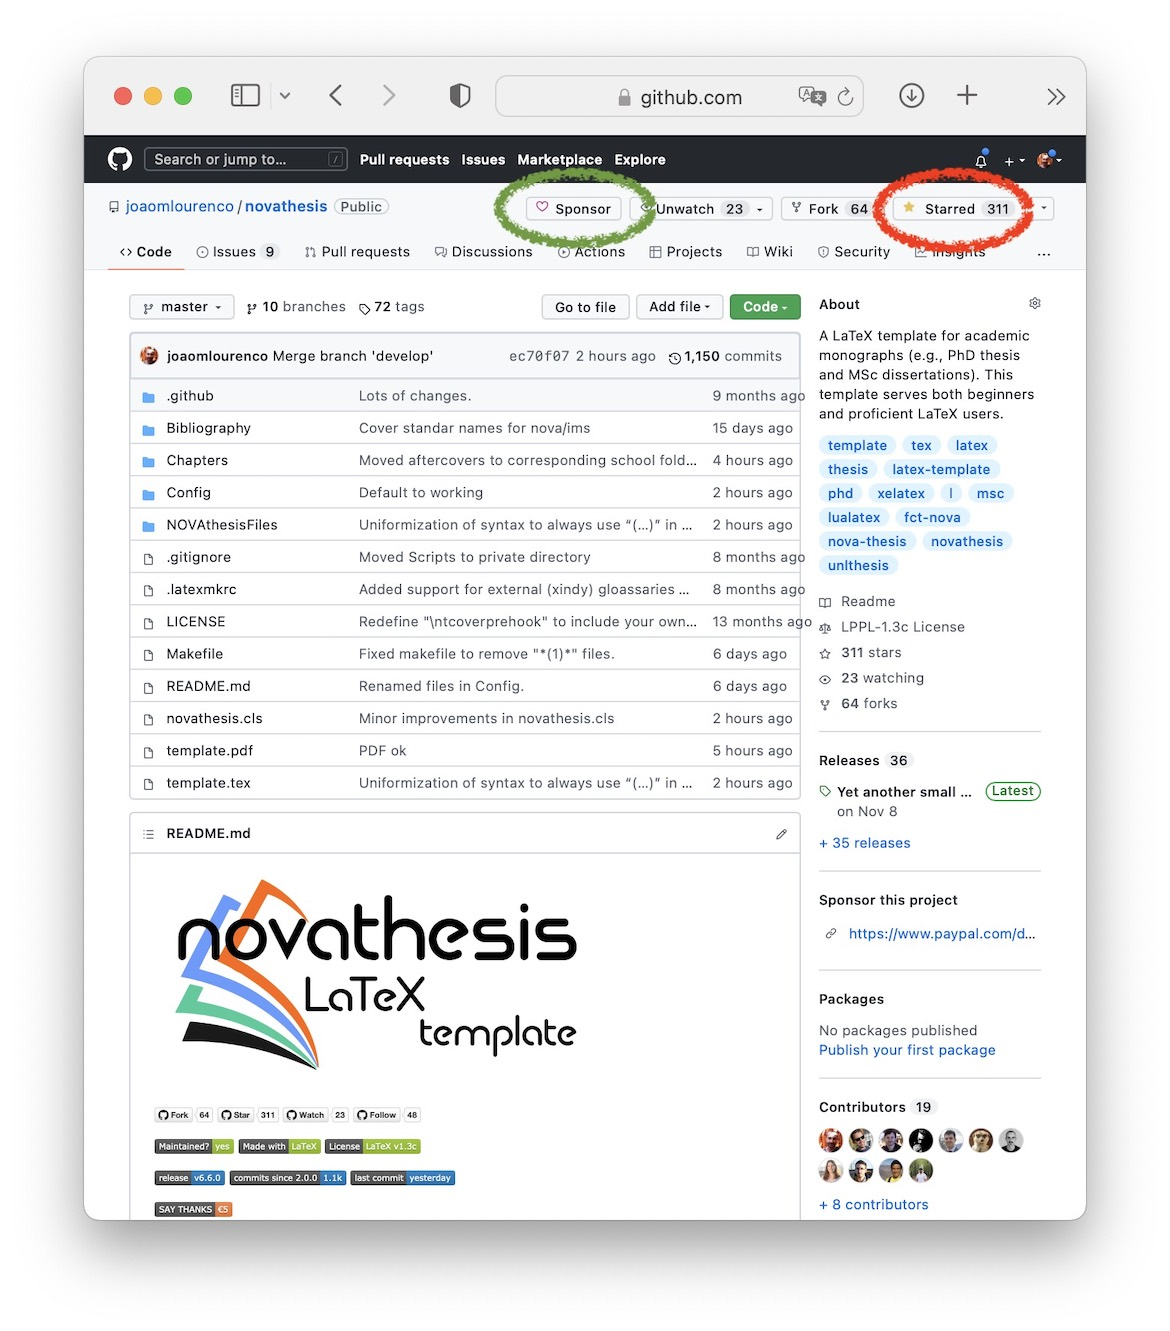
\includegraphics[width=0.5\linewidth]{github1}
    \caption{The \gls{novathesis} project web page in GitHub.}
    \label{fig:github}
\end{figure}

\section{Solução Proposta}
\label{sec:solution}
